This chapter discusses related work in the field of digital preservation.
First some general information about projects and activities are presented, and then an overview of the most common techniques of dealing with digital content in the long-term are outlined.
Then a definition of the term collection is given and important aspects such as meta data analysis and scalability are discussed.
Subsequently the chapter gives an overview of the current state of the art in tool support and discusses the influence and importance of quality assurance of measurements with respect to content profiling.
At the end, we draw observations about the state of the art and the identified problems and gaps.

\section{Preservation}
More and more information is produced in digital form and has only a digital representation.
This has enormous implications for national and state archives, libraries, scientific institutions and business enterprises, but also the small companies and even private people, as they often face data corruption and access problems in the long term.
In general, digital preservation (or DP for short) copes with two main problems; preserving content (bit streams) for longer periods of time, and ensuring these contents are accessible and understandable in the future.
When talking about ``the future'' or ``longer periods of time'', informally we mean: ``as long as the content is needed''. This abstract definition of ``Time'' and ``Long Term'' can be more formally defined by the time needed for a changing technology to have a considerable impact on the data or the time for the requirements of the user community to change. This time span can be indefinitely long. \cite{citeulike:1971545}.
That is the reason why the field of DP is full of challenges. These span from the fundamental technical problems through organisational and social issues to practical and financial ones.

A good example to picture the problem and challenges in DP is presented in \cite{Lorie:2001:LTP:379437.379726} and in \cite{Rauber:2009:dpchallenges}. Imagine a file created today on a specific physical machine. This file is nothing more than a series of bits shaped in a specific format. In order to access this file in the long term, not only the bits and bytes have to be preserved but also the way of interpreting them (the format specification). This would also require preserving the programs that can open, render and manipulate the file, which in turn will require the preservation of the dependency libraries and software packages as well as the operating system and the whole environment in which these programs or program versions run. Failing to preserve only one single part of this chain, the content would be lost (even if the physical bit stream is still in tact). Heslop et al. look at this problem from a different angle and introduce the term ``performance''. The distinction between an article or newspaper in its paper form and its digital record representation is that the digital record is the result of the interaction between technology and data as opposed to the physical counterpart. This implies that the experience of the digital object only lasts during this interaction and that each rendering of the record is actually a new original copy of itself. If two or more agents render the object they should experience equivalent performances of this particular record. As a result the term 'original' does no longer refer to the original paper document but to the original performance of the particular record on a screen or a device where it was viewed \cite{nla.cat-vn3423702}.

Due to this and many other problems, a community of preservation experts has emerged.
Through the last decade a number of DP-related research projects and initiatives have been established.
These have identified problems and threats and have advanced the state of the art in this filed.
Starting in the mid nineties, scientists recognised that these problems could lead to disasters and thus the need of digital preservation and its importance.
By the beginning of the new millennium there were the first initiatives and projects in the EU that started focusing on research topics related to DP. These projects (ERPANET\footnote{http://www.erpanet.org/}, DELOS\footnote{http://www.delos.info/}, DPE\footnote{http://www.digitalpreservationeurope.eu/}) were aiming the establishment of a community, identification of target groups and transfer of expertise.
The first scientific research was focused on topics such as standards, system concepts, selection and appraisal policies and format identification. Ioannidis et al. suggested a reference model for digital library management systems describing the characteristics of such information systems in \cite{delos:refdlms}. Rauber et al. defined a testbed framework for documenting the behaviour and functionality of digital objects and preservation strategies. The main goal of the framework was to find possibilities to automate preservation experiments \cite{delos:frmdoc}. All this set the foundation for more technical and practical approaches that were undertaken in later projects (PLANETS\footnote{http://www.planets-project.eu}, CASPAR\footnote{http://www.casparpreserves.eu}). The aim of these was to research the preservation of simple digital objects such as office documents and images. These projects advanced the state of the art of digital preservation and, as a result, different tools and languages that automated important DP processes were developed. PreScan, for example, maintains and preserves objects' meta data in an automated fashion\cite{Marketakis:2009fk}. Becker et al. proposed a generic XML language for characterising objects to support digital preservation. The language aimed to support automatic validation of document conversions by decomposing the documents structure and representing it in a generic XML language \cite{Becker:2008uq}.
All this helped the establishment of a solid community and a body of expertise.
An overview of the EU DP projects and activities is presented in \cite{strodl:2011:dpreport}.

Present initiatives include more fundamental research that tries to focus rather on more complex and interactive objects than simple documents and data structures. Projects such as LiWA\footnote{http://www.liwa-project.eu} attempt to solve issues related to Web Archiving, whereas projects such as TIMBUS\footnote{http://timbusproject.net} and WF4Ever\footnote{http://www.wf4ever-project.org} focus on the preservation of business processes and scientific workflows. Galushka et al. outline a complete framework for preserving a business process with all its relevant aspects and dependencies in \cite{galushka-ipres2012}.
Other projects such as SCAPE\footnote{http://scape-project.eu} build upon the solid framework established in the past and aim to improve the state of the art of DP by developing infrastructure and tools for scalable preservation actions and integrating them with automated policy-based preservation planning and preservation watch systems and workflows. Schmidt presents the design of a preservation platform architecture that supports distributed algorithms and fits into various digital preservation use cases in \cite{schmidt-ipres2012}. Faria et al. present the architecture of a novel preservation watch system that monitors specific preservation related properties of different sources and notifies interested parties when important or critical events occur in \cite{FariaPDBFR12}.

\subsection{Common Techniques}
Through the years many tools and procedures were developed in order to preserve digital content. In the literature there are often different names for the same or similar concepts. Here we present the most prominent ones and try to differentiate them and put them in perspective. There are different levels of concern: physical, logical and semantical.
The physical level of concern deals with the data integrity, or in other words the correct storage of the bits and bytes. The logical preservation deals with problems such as their structure, formats, etc., and the semantical level copes with the problems of preserving the meaning of the encoded information. As the focus of this thesis is not much related to the semantical level, we will concentrate on the first two. \newline

\textit{Physical Preservation}\newline
Migration is the technique of copying, moving or converting some source of information to another target. In the sense of physical preservation, it is the concept of moving the bits to a different medium with a different (physical) location. There are many different media that can store digital data. Some are more stable than others; some are more popular than others. No matter what type of medium is chosen for data storage (CDs, DVDs, Hard Drives, etc.), it is not guaranteed that the data stream is safe. Through physical damage, bit rot or other disasters, there is a high chance that your digital storage media will fail to reproduce your bit stream. Thus on this lower level the only option would be to copy the streams to a different medium from time to time. This is strategy is also often referred to as \textit{refreshing} \cite{Lee:2002:SOTADP}.

However, refreshing the data does not guarantee that it will be accessible in a later point in time, as new media are also error prone. Therefore, approaches like LOCKSS (Lots Of Copies Keep Stuff Safe) \cite{reich2001lpw} make use of the distribution of many independent copies. Developed at the Stanford University, the LOCKSS approach was implemented in a librarian software system that deploys many low cost copies of persistent web-caches and enables the detection and repair of damages based on voting in opinion polls \cite{Maniatis:2003:PPR:1165389.945451}.
%eventually say other projects that use LOCKSS (ExLibris, JISC, Hoppla, etc.)
Following a LOCKSS approach, however, only minimises the risk of losing data. If there is no effort spent in management of the copies, then it is fairly easy to lose track of the copies. For a software tool this might seem irrelevant, but for a private user this is a real issue.

Furthermore, even if enough, well-managed copies have been stored and the data stream has been preserved, there is always the issue of software obsolescence and thus failure in the access and interpretation of the stream. A good example of this problem can be found in this blog post\footnote{http://unsustainableideas.wordpress.com/2012/10/15/ppt-4-adventure-learning/}) by the former head of the UK's Digital Curation Centre\footnote{http://www.dcc.ac.uk} Chris Rusbridge, who struggled to open and successfully read almost 15 years old PowerPoint presentation slides. \newline

\textit{Logical Preservation} tries to cope with the structural integrity of a digital object and how the data should be interpreted in order to render the encoded information of an object. It tries to deal with the problems of old and outdated formats and software. In order to preserve not only the bit stream, but also to ensure the integrity of a digital object and its successful interpretation in the long-term, another type of migration is often used \cite{Lee:2002:SOTADP}. New operating systems, new software tools or new versions are sometimes incompatible or unable to render and manipulate older formats. To cope with technology changes, digital preservation often uses a conversion strategy where the data is migrated (moved) to another format that is usually considered to be more stable than the original. A format is usually considered worthy and stable for preservation purposes when it is standardised, the format specification is open and well documented and there are no patent owners and license fees that apply. The Florida Center for Library Automation, for example, offers a report\footnote{http://fclaweb.fcla.edu/uploads/recFormats.pdf} with the recommended data formats for preservation purposes that is considered as a good reference and starting point. 

However, there is no ultimate reference table or no ultimate file format that fits all preservation purposes. From use case to use case, different aspects have to be considered. Neither standards, nor migration tools alone can ensure that a digital document remains accessible and its integrity remains unharmed. The format is only the tip of the iceberg, as the problem is various and manifold. In the end, there are always many different aspects that have to be considered and it always comes down to a multi-criteria decision making problem \cite{becker:decision}.

Wing and Ockerbloom further discuss the topic as they analyse what information is preserved by type converters and formalise the notion of respectful type converters in \cite{859529}. Informally, a migration tool (or a converter) respects a certain type T if an original object A and a converted object B show the same behaviour when viewed as objects of type T.

Rothenberg gives a good overview of common flaws of the concepts of migration in \cite{rothenberg:1999:ensuring} and summarises important aspects that should be considered in DP. For example, the translation to a new format has the flaw that the original is usually discarded afterwards (e.g. because of storage costs). This can make it impossible to validate, whether or not information has been lost.

Nonetheless, format migration is often applied within digital preservation systems and repositories. As it also has potential pitfalls, it is not to be taken lightly.
A more practical downside to migration is the storage cost. Often the target format has a bigger footprint than the original. Also the conversion of huge amounts of data is an error prone process that is not easy to validate \cite{Lorie:2001:LTP:379437.379726}. Thus the originals are often kept for a certain period of time after the migration. Furthermore, if the migration path consists of several steps one, has to make sure that all required meta data of the original is also migrated to the new versions of the objects. Another related issue is also quality assurance. As it is infeasible to check manually if the conversion process was successful, there are very specific requirements and processes that have to be followed in order to automate the verification of the preservation action \cite{feng:2010:qrofm, becker:decision}.
All these and other issues have to be carefully taken into account before choosing such a preservation action.
\newline

Another common technique of logical preservation is emulation. It has the verb ``emulate'' in its root and means to imitate or reproduce.
In software terms, an emulator is a software tool that imitates the behaviour of a (hardware) system/framework (usually an older one) in order to run other (obsolete) tools that are meant to run on the emulated system. Clearly, this approach can come in handy in some DP activities.
In \cite{rothenberg:1999:ensuring} Rothenberg gives an overview of a process for preservation that is based on an emulation process. The author states that not only the data (bit-stream) has to be stored but also the bit stream of the original program, the operating system and all other necessary parts, e.g. dependencies and used libraries. Also a thorough and complete description and specification of the underlying architecture have to be provided in a form that is readable by potential future emulator authors. If these prerequisites are met, an emulator that mimics the specific hardware needed to run the tool can be created.
Lorie points out in \cite{Lorie:2001:LTP:379437.379726} that the specification of the architecture has to be perfect and complete, which is an immensely difficult task. Another very important argument he makes is the evaluation of such an emulator. Even if all needed input existed and a hypothetical emulator was created, how can its correctness be proven as no original hardware device exists?

These and other reasons combined form one of the biggest downsides of emulation; cost. The effort, manpower and infrastructure needed to emulate an environment that renders digital documents is often more expensive than the value of the content of the documents themselves.

Nevertheless, emulation is widely used in specific branches, such as video gaming.
Guttenbrunner et al have evaluated different strategies for the preservation of console video games in \cite{guttenbrunner:2008:evaluating} and came to the conclusion that while migration shows very good results for the preservation of visual and audio components, it completely fails in interactivity. Emulation, on the other hand, showed promising results. All of these, however, were strongly dependent on the sample objects that were emulated. Some of the evaluated emulation alternatives worked great on some of the sample records but completely failed on others, which is an important aspect to keep in mind when selecting representative objects and stresses the importance of the way these are selected.

\subsection{Preservation Planning}
\label{lbl:preservationplanning}
Preservation planning is a key task in DP that has to be undertaken by every institution or person that is serious about preservation. Numerous DP related projects have investigated the key requirements and processes involved in preservation planning. Projects such as PLANETS\footnote{http://www.planets-project.eu/} have created very strong fundaments in this area and have developed tools such as PLATO\footnote{http://ifs.tuwien.ac.at/dp/plato} - the preservation planning tool which supports a standardised workflow and helps users throughout numerous steps with the goal of creating a preservation plan. Follow up projects, such as SCAPE\footnote{http://www.scape-project.eu/} advance the state of the art and enhance the planning capabilities by improving the current status. This involves building up a framework around the process that supports many new features such as preservation monitoring services, semi-automatised experiments execution, automatic plan deployment and execution and many more enhancements to the whole process in order to provide a scalable, robust preservation planning process.\newline

\noindent\textit{What is Preservation Planning?}\newline
The OAIS reference model was developed by the Consultative Committee for Space Data Systems and soon afterwards was accepted as an ISO standard \cite{iso:2003:oais}. This high-level reference model has proven to be a helpful tool for the DP community for many years. Undoubtedly, one of its key parts is Preservation Planning or PP for short.

At the core of PP is the recommendation of archival operations. This requires a decision making process that evaluates different preservation strategies or actions and chooses the most appropriate one. The outcome of the process is highly dependent on object characteristics and institutional settings and requirements \cite{STR07_jcdl}. The goal of the process is to create a preservation plan that documents all the steps and choices that were made, the policies that were followed while making these decisions and the different preservation alternatives that were evaluated. It offers a complete documentation of the decision that allows one to repeat all experiments and verify why a certain preservation action was chosen at a given point in time.

\begin{figure}[th]
\begin{center}
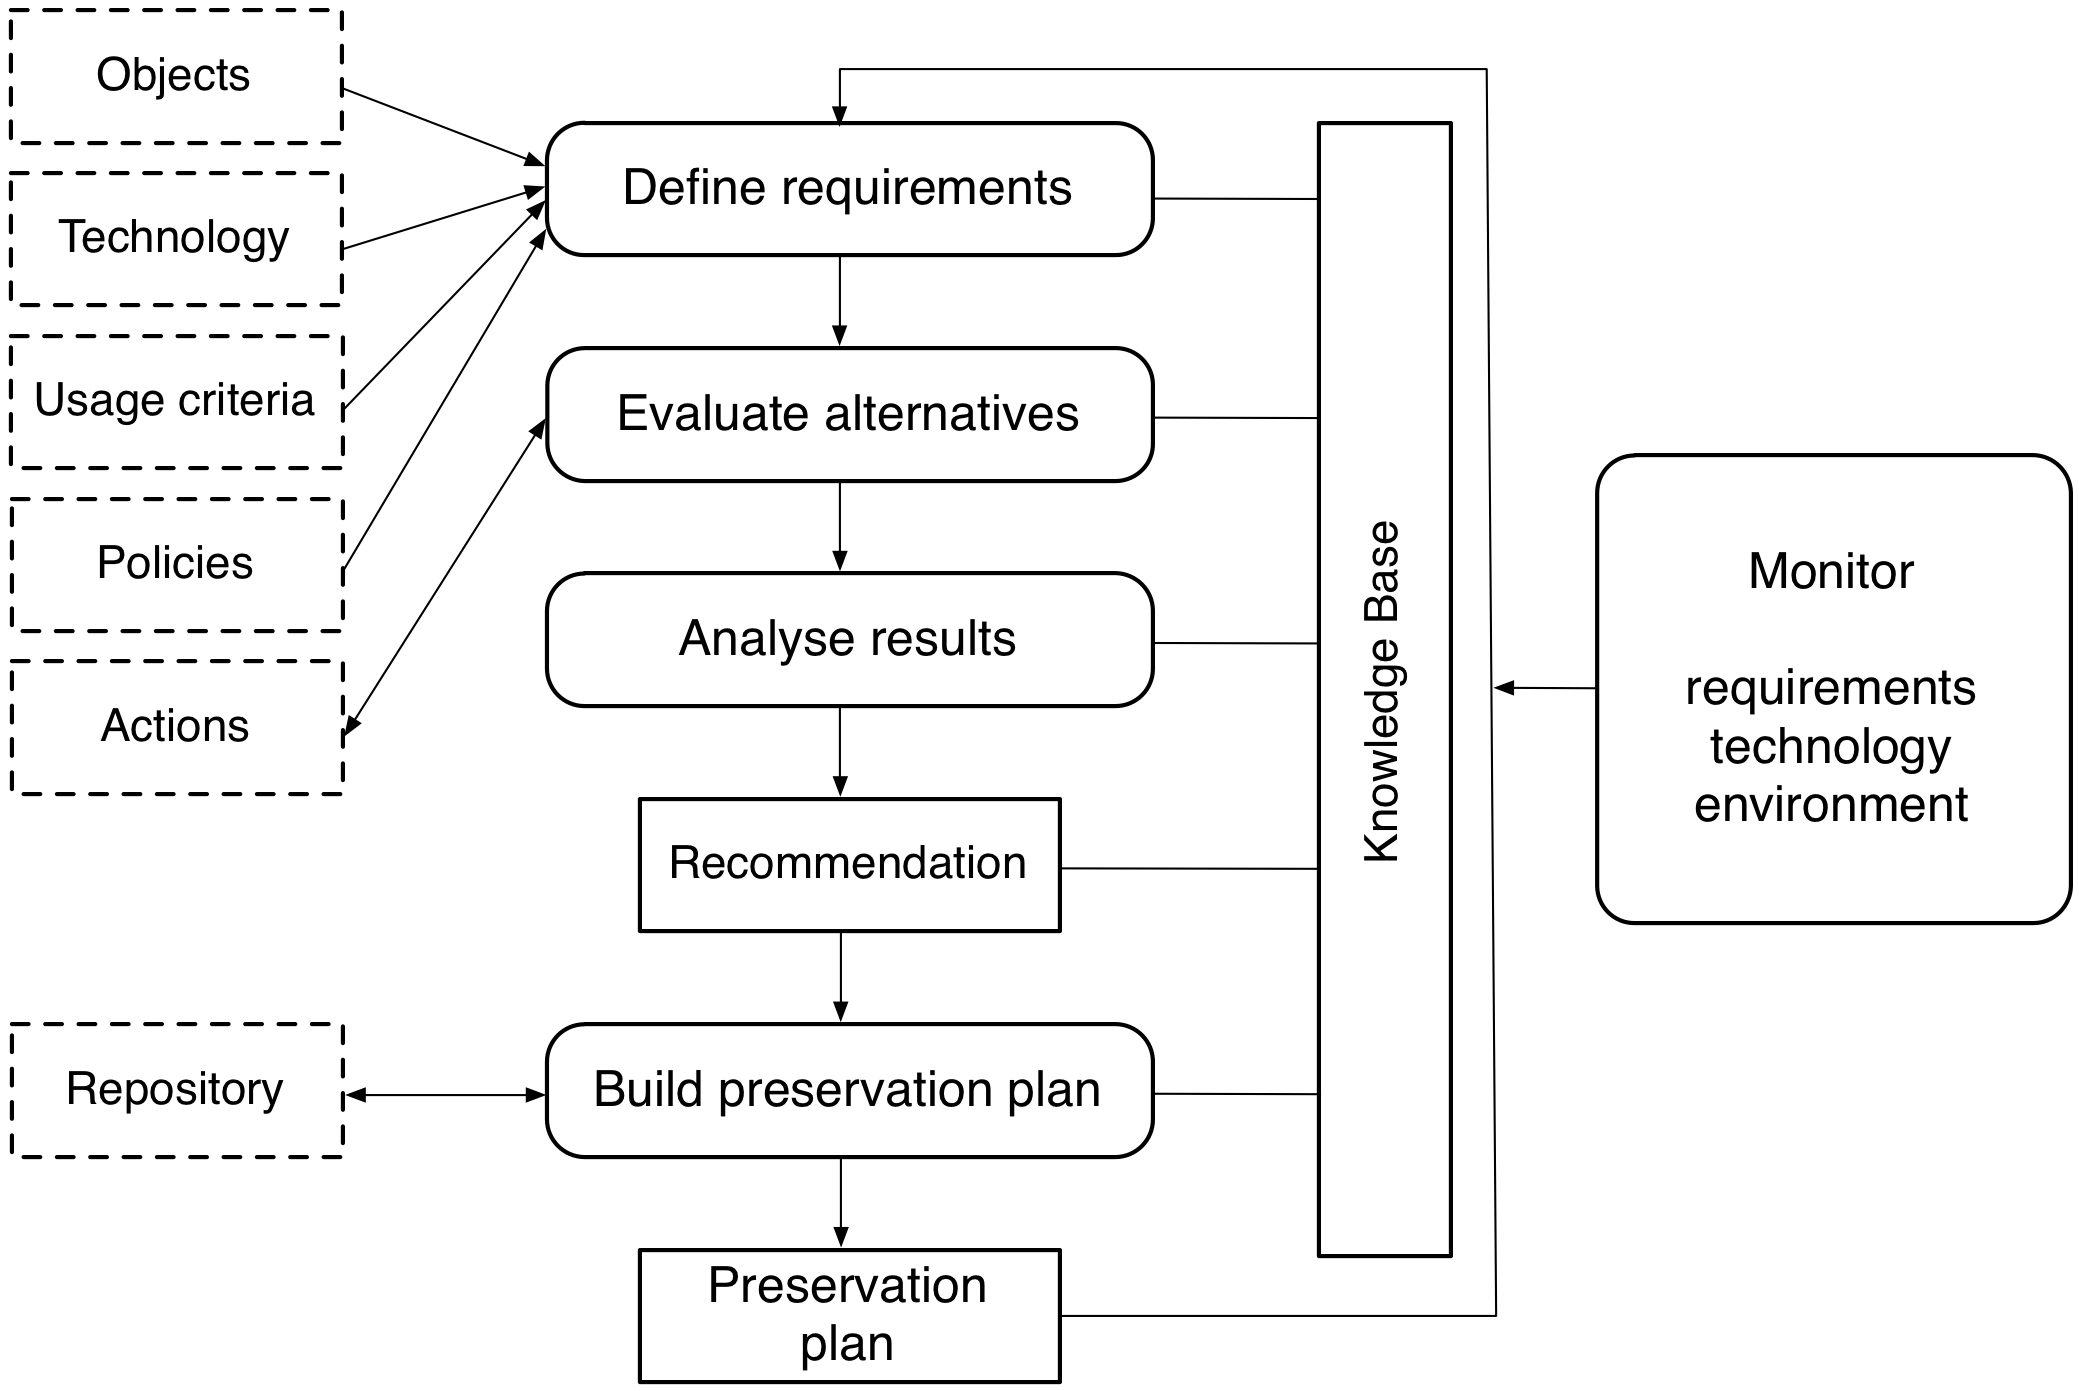
\includegraphics[width=4.5in]{figures/related/planningenvironment.png}
\caption{The preservation planning environment \cite{Becker:2009fk}.}
\label{fig:planenv}
\end{center}
\end{figure}

Figure \ref{fig:planenv} depicts the planning environment of the whole planning process. It constitutes of four main phases: define requirements, evaluate alternatives, analyse results and build preservation plan.

In the first step, all necessary requirements for the specific use case are collected. This includes the identifiers and a profile of the objects or the collection that is examined, but also the technical environment and specific usage criteria for the particular set of objects. Another important part are the organisational policies, which are usually high level statements that guide the organisation.

In the next step, different alternatives are evaluated. These are called preservation actions and implement different preservation strategies, depending on the use case. Depending on the chosen
strategy, different preservation action tools can be evaluated by conducting different experiments over a set of objects. As every strategy offers a set of tools and every tool has its own set of configuration parameters, this step may become quite expensive in terms of time and resources.

As soon as the experiments are conducted, a planner has to analyse the results objectively and decide which of the tested actions makes most sense considering the requirements and the experiment results. It is important to note, that
keeping the status quo is a perfectly valid solution in many use cases and is also supported by the planning process.

After a recommendation is made, a preservation plan is created, which is a very concrete artefact, as opposed to policy documents, that specifies an action plan for the preservation of a set of digital objects.

\begin{quote}
\textit{A preservation plan defines a series of preservation actions to be taken by a responsible institution due to an identified risk for a given set of digital objects or records (called collection). The Preservation Plan takes into account the preservation policies, legal obligations, organisational and technical constraints, user requirements and preservation goals and describes the preservation context, the evaluated preservation strategies and the resulting decision for one strategy, including the reasoning for the decision. It also specifies a series of steps or actions (called preservation action plan) along with responsibilities and rules and conditions for execution on the collection. Provided that the actions and their deployment as well as the technical environment allow it, this action plan is an executable workflow definition}\cite{Becker:2009fk}.
\end{quote}

Since planning is not a one-time activity, there is also an external monitoring phase that keeps track of important preservation related aspects of the world, such as new technology, formats and the organisational policies. It feeds back this important information about relevant changes in the environment, which can cause a reiteration/re-evaluation of a preservation plan. A detailed overview and a high level design of such an addition to the preservation planning environment can be found in \cite{duretec:2012:watch}.

As content profiling is a very important and necessary part for efficient and successful preservation planning, we take a look at the whole process in detail in order to understand where profiling fits in the process and how can it help enhance it later. It is a well-defined workflow consisting of four phases with several steps which are discussed in \cite{STR07_jcdl}.

In the first phase, \textit{``Define Requirements''}, the scope of the preservation plan is demarcated. The preservation expert has to follow three steps; to provide information about the collection, environment etc. (\textbf{Define Basis}), to choose representative sample records for experimentation (\textbf{Define Sample Records}) and to identify the requirements for the preservation plan or the so called objective tree, which summarised high-level goals of the plan (\textbf{Identify Requirements}). 

In the second phase, \textit{``Evaluate Alternatives''}, another 5 steps have to be followed. Starting with the definition of alternatives (\textbf{Define Alternatives}), the responsible preservation expert has to choose a set of potential actions, with all related information such as environment, tool invocation parameters, etc. In the following (\textbf{GO/NO-GO}) step a decisions is made whether to proceed or not based on each preservation action, the estimated resources and the defined requirements. After that the planner has to create suitable experiments (\textbf{Develop Experiment}), which are well-documented, repeatable set of actions with their environment and the capability to capture their results. In the following (\textbf{Run Experiment}) step, each preservation action is executed against the chosen sample records in order to obtain different results. In the last step of this phase (\textbf{Evaluate Results}) the results of the experiment output is evaluated against the objective tree in order to check if the identified requirements were met or not.

The third phase, \textit{``Consider Results''}, is responsible for the objective analysis of the results. In its first step (\textbf{Transformed Measured Value}) all experiment results are transformed into the same scale (0-5) making use of special transformation tables and utility function. The following (\textbf{Set Importance Factor}) step provides the ability to equal the weight of different parts of the requirement objective tree, as not all goals are equally important. In the last step (\textbf{Analyse Results}) all measures are aggregated per objective and provide the planner with a preservation action recommendation and the necessary basis for a decision.

\begin{figure}[tbp]
\begin{center}
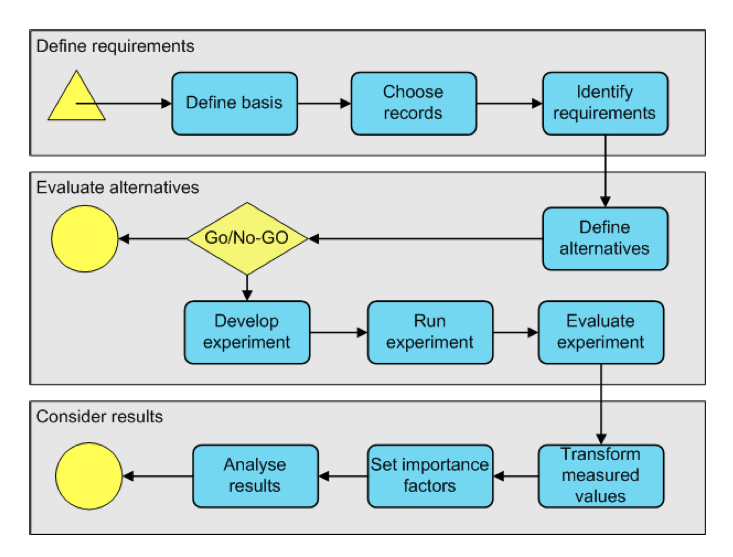
\includegraphics[width=5in]{figures/contentprofiling/planningworkflow.png}
\caption{Overview of PLANETS Preservation Planning workflow \cite{Becker:2008:PSO:1378889.1378954}.}
\label{fig:planningworkflow}
\end{center}
\end{figure}

The workflow is depicted in figure \ref{fig:planningworkflow} and provides the current state of the art in preservation planning matters. Although it provides a very solid theoretical ground and a complete specification that is working in practice, there is one part of the concept, which might be the cause of errors caused by human incompetence or lack of knowledge and understanding of the collection.

As one can see from the workflow, all the results strongly depend on the defined goals and the analysis of the experiments output. We assume that a preservation expert will understand the objectives of his organisation. Since the identification of requirements and the setting of the goals and objectives are very important steps that are also strongly dependent on the organisational background of the preservation expert, we also assume that it is unlikely they will cause errors and misunderstandings in later steps. Also if the planner happens to choose wrong preservation action alternatives, the result will be in the worst-case scenario a 'Do Nothing' alternative, which will not solve the problem at hand, but will also not do any damage.
However, there is one step that could have serious implications and even cause damage or at least resource loss if taken lightly. Consider the following example, where the chosen sample records are picked up at random from a medium sized collection with several thousands of objects. Then the experiments show a particular preservation action is very feasible and the planner chooses to execute this action over the whole content, due to the experiments output and the consequent analysis. Although the analysis and the decision are perfectly valid (in their implementation and execution), it could turn out that the result of the preservation operation does not meet the requirements defined. This could happen, due to many different aspects in the format and content profile of the collection at hand. To summarise, the defined requirements and objectives are ok, the experiments are valid, the analysis is correct, but the overall results are not feasible due to the false premise, that the random chosen set of sample records is representative. Damage could be done, if there is no reasonable and thorough quality assurance process afterwards. This work addresses this problem and tries to prevent it by reducing the bias of the experiments. This ought to be achieved by thorough analysis and automatic representative selection in the early steps of the workflow.

One can argue, that no real preservation expert will choose representatives at random. Although this might be true, there are numerous other factors that have to be considered when choosing the representatives and since the collections that are worth preserving are often big enough, the overhead for the preservation expert is just not feasible to select them by hand. Thus the representatives are usually chosen by format and format version in combination with their size (minimum, maximum and average).

The planning tool PLATO, developed at the University of Technology in Vienna, implements this process and appends a fourth phase, where the user/planning expert can create an executable plan, which can be deployed within a repository. 
This fourth phase, (\textit{``Build preservation plan``}) adds an important part to the workflow and results in an applicable real world preservation plan artefact. The preservation action plan is a well-defined specification that serves the purpose of documentation of the decision and contains the executable part, which specifies the tools, environment and parameters to use during the preservation operation.

However, in its current release, the planning tool supports only manual sample records definition. Although it assists the planner with integrated characterisation tools, it cannot provide higher certainty in the validity of the chosen representatives. Integration with another tool that provides a complete content profile (generated in an automatic fashion) would provide a huge benefit to preservation planners.

\section{Content}
As seen in the previous section, understanding the objects in a collection is a key part of the requirements for preservation planning. In order to create and analyse a collection or a set of digital objects, the meta data for each object has to be examined. Meta data is structured information about the data (objects) itself. It is usually stored within a file that provides further information about the content and format of the file as well as other important characteristics. In general, there are three main types of meta data: descriptive meta data for discovery and identification (e.g. title, author, etc.), structural meta data (page ordering, image width and height, etc.), and administrative meta data that helps management of the resource (e.g. creation date, type, etc.). The National Information Standards Organisation - NISO\footnote{http://niso.org} has provided a series of articles and reports in order to help people, archivists and experts understand meta data and its importance \cite{citeulike:6387279}.

Today, analysis of such huge content often is done in a manual fashion, which can be a very time-consuming and cumbersome task. If there would be tools at hand that support identification and characterisation, data aggregation, filtering, collection splitting, etc., then the analysis process will be automated to a certain degree, hence analysis will be handled much faster and potentially much more efficient. 

It is noteworthy that content here neither refers to the semantics of the information stored within the digital objects, nor to their visual representation characteristics or anything similar, but solely to the digital artefacts and the definition of the collection in terms of meta data, such as formats and format-related characteristics.

Consider a collection of digital scans of old newspapers. Its content here does not refer to the content of the newspaper articles, but to the meta data characteristics of the images that comprise the collection. For example, these may include, but are not necessarily restricted to the resolution of the scanned documents, their colour profiles, the size of the images or the number of pages. All these measurements play a huge role in the decision making process of preservation planning.

The following paragraphs provide more details on metadata and how this refers to content profiling for preservation planning.

\subsection{Identification vs. Characterisation}
Identification is the process of determining the format of certain sequence of bits and bytes. It is an important aspect not only for DP, but also in many other fields of computer science. Thus, there are numerous different methods of identifying the format of a file.

A trivial and popular approach is based on the extension of a file, or in other words the end of the file name. Many (early) versions of different mainstream operating systems use this approach. Unfortunately, it is rather flawed and unfit for DP for a number of reasons. For one, software or user clients easily manipulate the extension. Also, many files do not have an extension. Another problem is, that sometimes file formats produced by different software applications have the same extension.

A more sophisticated method for identifying a format of a file is by using its internal meta data. For example, this can be done by examining the file header (the beginning of the byte stream of a file) information. Many formats start with a few special bytes (called magic numbers) which define the following format \cite{linfoproject:magicnumbers}. Some tools make use of magic number tables and identify the format by comparing its magic number and table. Magic Numbers are a better solution than file name extensions, as they are harder to manipulate. The problem is that often magic numbers are not well documented and are easily lost. Furthermore, the tables used for comparison have to be maintained.

Characterisation, on the other hand, is the process of extracting more meta data out of the file, that can help explain the file, provide related information, such as the language, author, creating date, etc. Based on the different measurements of properties/characteristics a collection can be dubbed homogeneous or heterogeneous. Usually to a user a homogeneous collection would be a set of files that consists only or mostly of objects having the same format or even the same type (audio, video, text, etc.). This, however, is an oversimplification, which has enormous side effects for preservation planning.

Consider a collection of N digital objects, which share the same extension, e.g. 'pdf'. To a normal user, this would be a homogeneous collection. An advanced user, however, would know that the extension of a file does not really specify the format of the file and thus could assume that there are differences.
One step further would be to conduct an identification process that looks for the specific file format and format version. Assume that in our example 95\% of all files have the same \textit{PDF} format and format version.  Then this could be considered a homogeneous collection with respect to the format.  In a next step, however, characterisation is conducted and now there are many more properties, such as \textit{creating applications}, \textit{encryption}, \textit{password protection}, \textit{tags}, etc.
Regarding these characteristics, the same collection can be considered to be heterogeneous.
Clearly, all of this is very important to preservation planning, since different preservation actions produce different results exactly because of big differences in the values of such characteristics.

Thus the question remains, how to identify such important properties that define the homogeneity of a collection? Following this train of thought, clearly the format is a very important characteristic. However, it does not cover all cases (as in the example) and many others are important.

\subsection{Preservation Analysis}
As collections in DP are often just too large for a human being to comprehend, the meta data provided by identification and characterisation has to be aggregated and analysed in some fashion. For this purpose different statistical information is used to understand and stratify the content into different homogeneous parts. Often simple statistical measures about the size, such as minimum, maximum, average, standard deviation, etc. provide meaningful information about the current content one has to deal with. Moreover, histograms and distributions of mime types, formats, format version and other properties help to see the bigger picture of the content that is to be preserved.

Once the bigger picture gets clearer, the collection can be divided into different (more) homogeneous parts, which will ease the decisions that have to be made regarding their future with respect to DP and PP. In order to achieve this stratification, filtering or so-called slicing and dicing has to be applied on the data. This would include the traversal of the raw data and splitting the content into sets.

Another important part would be finding representatives within the homogeneous content. These are very small sized subsets (usually in the order of tens of objects) that are somehow representative to the selected content or part of it. The representativeness can be determined based on the distribution of different characteristics or combinations thereof. These representative samples form a better-suited common ground for the experimentation phase of the preservation planning process. Finding such small subsets within homogeneous collections is potentially much easier than in heterogeneous context. 

Automating the retrieval of such a set is not a trivial task, as there are numerous factors to consider. Pan et al. discuss the topic in \cite{Pan05findingrepresentative} and propose an approach for finding representatives in a massive data set by building a distribution table of different content features. The presented algorithm relies on an objective function that is not well specified, but gives a good overview of the complexity of the task.

The problem of representativeness will be investigated in later parts of this thesis. The next chapter defines some informal requirements that a sample object set has to meet. Chapter 4 presents a small set of simple algorithms that are able to find representative objects in a collection based on different criteria. The aim is to identify potential problems and allow future work to build upon these and create more complex and sophisticated algorithms.

\subsection{Scalability}
As discussed in Section \ref{ch:content_and_digital_preservation}, content growth nowadays has a tremendous pace. This fact has some serious implications on how information systems have to deal with it. Scalability does not only pose a problem related to volume and performance, but also to usability and presentation, automation and costs.

Looking at the growth of content within web archives, for example, and their projection the problem of vertical scalability becomes clear. Vertical scalability (i.e. installing machines with better performance) will not be able to solve the problem of storage and data management, not to mention the effective analysis of data.

Since this is a problem not only related to digital preservation but to information systems in general, there are many studies for algorithms, technologies and architectures that enable horizontal scalability, i.e. attaching more commodity machines and distributing the payload among them.

Driven by economies of scale, Cloud Computing has played an enormous role in this area by providing a large set of easy to use and access resources, such as hardware, development platforms and services \cite{Vaquero:2008, 4738445}. Distributed Platforms as a Service (PaaS), such as Amazon AWS\footnote{http://aws.amazon.com} and Amazon S3\footnote{http://aws.amazon.com/s3/}, Google App Engine\footnote{https://developers.google.com/appengine/}, Heroku\footnote{http://www.heroku.com}, etc. have proven to be very performance- and cost-effective. Distributed approaches and algorithms, such as Google's Map Reduce \cite{Dean:2008:MSD:1327452.1327492} have found many applications in various fields of computer science. 

Map Reduce is a fairly modern parallelisation algorithm for processing large data sets on certain kind of distributable problems. The framework can make use of a large amount of nodes for the computation. It takes as input a set of key/value pairs and produces a set of output key/value pairs. It typically consists of only two functions: map and reduce. In some cases a third finalize function can be used to do some further computation that needs all the results of the reduce steps.

The Map function takes a set of pairs of keys and values in the form of (k1, v1) and transforms them to a set of intermediate key/value pairs. The framework groups together the intermediate values by key and passes them for further processing to the Reduce function.

The Reduce function accepts an intermediate key and a list of values associated with that key and is responsible for computing the (partial) final result. The reduce function can be invoked many times by the framework and there is no guarantee that it will be run on the same node as the Map function. This means it has to be idempotent and agnostic to external knowledge about the distribution.

This rather simple approach has been widely accepted by the OpenSource community and was implemented by the Apache Software Foundation in a library called Hadoop\footnote{http://hadoop.apache.org}. The possibility for integration with a BigTable-like Store \cite{Chang:2008:BDS:1365815.1365816} (HBase\footnote{http://hbase.apache.org}) and a distributed file system (HDFS\footnote{http://hadoop.apache.org/docs/hdfs/r0.22.0/hdfs\_design.html}) has enabled many companies to handle the big volumes of data they have. Google was using a similar architecture for its index construction, article clustering and statistical machine translation. Yahoo uses it for spam detection in its mail service and other big corporations use it for data mining, ad optimisation and more.

All this sets a solid foundation for in-depth analysis of meta data on larger scales, which would greatly help planners to automatise the content profiling and preservation planning processes. Furthermore, planners will benefit from the fact that such technology will increase performance and most likely provide more efficient results.

\subsection{State of the Art}
Observing the current state of art implies that analysis of preservation related data should be feasible and cost-effective. Nonetheless, preservation analysis tools nowadays often lack the ability to analyse content on a larger scale, or if they support it, there is a trade off in the analysis depth. This fact is due to two common worldviews. On the one hand, there is the popular belief that the format is the one property that matters for digital preservation \cite{citeulike:8904907} and that there is no real need to look at many different aspects. On the other hand, the volume of the data is so high, that even the deep characterisation meta data volume can be considerably large, which impends large-scale analysis. These observations of the current state of the art of preservation analysis approaches are sketched in Figure \ref{fig:sota_analysis}. 
The \textit{X} axis depicts the depth of the analysis of tools and frameworks in terms of considered characteristics.
The \textit{Y} axis depicts the volume of the meta data used for the analysis. The figure illustrates the trade off between large volumes of data and the number of identification and characterisation properties that can be analysed.

Another fact that contributes to the problem is that digital repositories often provide only simple metrics such as the format profile - an aggregation of the formats in the repository and their absolute occurrences, ingest and creation date and in some cases the applications. Even though the repositories often have the means to characterise the data or even store it, there is no easy way to obtain a bigger picture about a certain collection.
Often the only way to obtain more specific information that relates two or more characteristics out of a repository involves
issuing complex queries directly to the database of the repository. This is not user friendly and feasible to a planner, but also requires the knowledge of system administrators.

Last but not least, selecting representative sample objects is usually done manually. The chosen samples are often stratified based on size and format \cite{journals/dlib/KulovitsRKBBS09}. This might be enough, but there are certainly cases where looking at other characteristics and the combinations between is more important.

\begin{figure}[th]
\begin{center}
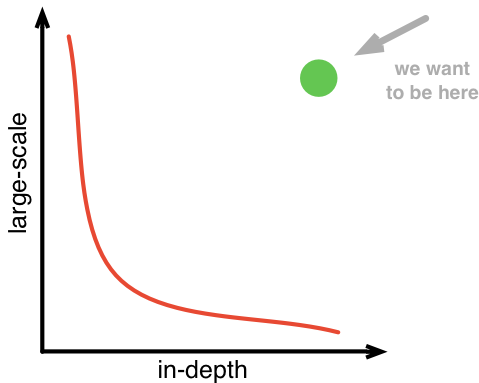
\includegraphics[width=3.6in]{figures/related/sota_analysis.png}
\caption{The current state of the art of preservation analysis tools and frameworks in relation to the volume of content and the depth of the analysis.}
\label{fig:sota_analysis}
\end{center}
\end{figure}

\section{Tool Support}
\label{lbl:tool_support}
%talk about meta data tool support
%preservation planning tool support and automation and scalability
%content profiling/ format profiling tool support
%repositories, monitoring services
Due to the rising awareness of digital preservation and the numerous projects conducted in this area in recent years, many existing tools have found new use and many new tools were written from scratch in order to support DP activities. This section provides a short overview of some of the more prominent ones that are related to content profiling.

A recent report (created as part of the SCAPE project) summarises an evaluation framework and the results of the tests of several identification and characterisation tools \cite{Knijff:2011it}. It provides a rather good overview of the current state of the art of such tools but concentrates mostly on their identification capabilities. In the report six tools (DROID 6.0\footnote{http://sourceforge.net/projects/droid/}, FIDO\footnote{https://github.com/openplanets/fido}, Unix File Tool\footnote{http://unixhelp.ed.ac.uk/CGI/man-cgi?file}, FITS\footnote{http://code.google.com/p/fits/} 0.5 and JHOVE2\footnote{https://bitbucket.org/jhove2/main/wiki/Home}) were evaluated against 22 criteria such as tool interface, its license type, platform dependencies, accuracy of reported results, documentation, etc. Another recent research conducted by the National Library of Australia has investigated four file identification tools (File Investigator Engine\footnote{http://www.forensicinnovations.com/fiengine.html}, Outside-In File ID\footnote{http://docs.oracle.com/cd/E16184\_01/dev.837/e12875/title.htm}, FIDO and file) and five metadata extraction tools (File Investigator Engine, Exiftool\footnote{http://owl.phy.queensu.ca/~phil/exiftool/}, MediaInfo\footnote{http://mediainfo.sourceforge.net/en}, pdfinfo\footnote{http://www.foolabs.com/xpdf/download.html} and Apache Tika\footnote{http://tika.apache.org}), some of which commercial. The results of these tests can be found in \cite{NLASP2452}.

Here we summarise the strengths and weaknesses of some of these and other tools briefly in order to give an overview of the current state of the art.

\begin{itemize}
\item \textbf{DROID 6.0}\newline
Droid is an identification tool produced by the National Archives, which uses the PRONOM\footnote{http://nationalarchives.gov.uk/pronom/} registry and its format signatures and/or file extensions. It provides information about the mime type, format and format version of a file as long it is in the DROID signature file, which contains the 'magic numbers' of the PRONOM registry. It also outputs a PRONOM Unique Identifier or PUID, which can be used to trace the format back into the registry.
Unfortunately, the registry is not open and its maintenance is slow. However, the tool is very useful and widely adopted within the DP community.

\item \textbf{Apache TIKA}\newline
Tika is an open source project from The Apache Software Foundation that is able to extract metadata from files with various formats. It is a stable tool able to identify files by analysing their bitstream and allows the deeper characterisation of some of these files.  

\item \textbf{FIDO}\newline
FIDO is another identification tool that is a clone of Droid and also uses the PRONOM signature file registry. Although it has numerous glitches, FIDO's performance proves to be 35 times faster than DROID when working on one file at a time.

\item \textbf{UNIX File Tool}\newline
File is a CLI utility application included in every Unix distribution and first released in 1973. The tool has stood the test of time and has proven to be very stable, which also makes it widely adopted in the DP community. It makes use of magic numbers to identify files and has been used in DP activities for a long time. It has a very good computational performance and supports large number of formats.

\item \textbf{JHOVE}\newline
JHOVE is one of the most well known identification and characterisation tools used by the DP community. It is also developed by the Harvard University Library and is able to extract meta data from various formats based on different modules. Probably one of the most valuable features of JHOVE is the ability the check a file for well-formedness and validity against the format specification. Figure \ref{fig:jhove_screenshot} shows a screenshot of JHove and the output of an example PDF file.

\item \textbf{JHOVE 2}\newline
JHOVE 2 is a successor project for the JHOVE tool and also provides an extensible architecture for characterisation tools and modules. It is developed as an open source tool by the California Digital Library, Portico and Stanford University. Currently it produces helpful output only for a few types of documents as the different modules are not yet developed.

\item \textbf{FITS} \newline
The File Information Tool Set is developed by the Harvard University Library. It wraps common identification and characterisation tools as the ones described here and tries to consolidate them and provide a normalised output. By providing basic provenance information for each extracted record, it combines the consolidation result and provides a very basic confidence status for the extracted value of each property. This proves to be helpful for cases where there are uncertainties. The framework is designed to be extended, so that other tools can be also added. The tool seems very helpful, although there are some instabilities and problematic cases. An example FITS output file is provided in Listing \ref{lst:fits_example}. Every FITS file consists of four sections: \textit{identification}, \textit{fileinfo}, \textit{filestatus} and \textit{metadata}. The 'identification' section provides information about the mime-type, format, format version and optionally external identifiers, such as PUIDs. The 'fileinfo' section lists some generic to the format characteristics, such as size and creation date. The 'filestatus' section gives information about the structure and the validity of the content according to the format. The last 'metadata' section lists all format specific characteristics for the characterised file.
\end{itemize}

\begin{figure}[th]
\begin{center}
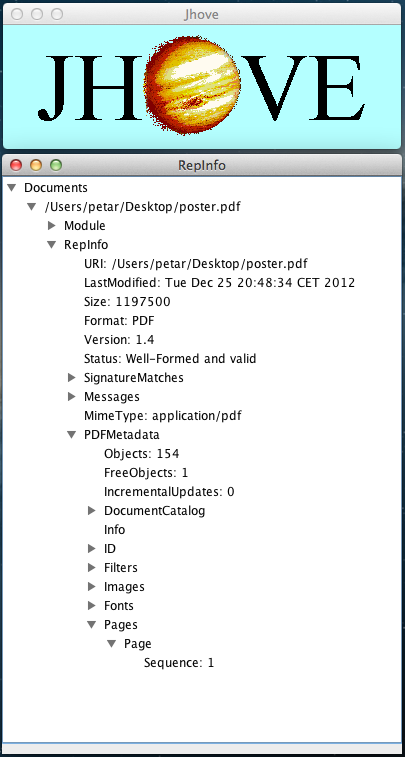
\includegraphics[width=3in]{figures/related/jhove_example.png}
\caption{A screenshot of JHove showing part of the output for an example PDF file.}
\label{fig:jhove_screenshot}
\end{center}
\end{figure}

\clearpage

\lstset{
language=XML,
basicstyle=\tiny\ttfamily,
label=lst:fits_example,
caption=An example FITS output file}
\begin{lstlisting}
<?xml version="1.0" encoding="UTF-8"?>
<fits xmlns="http://hul.harvard.edu/ois/xml/ns/fits/fits_output" xmlns:xsi="http://www.w3.org/2001/XMLSchema-instance" xsi:schemaLocation="http://hul.harvard.edu/ois/xml/xsd/fits/fits_output.xsd" version="0.6.0" timestamp="12/14/11 12:39 PM">
 <identification>
   <identity format="Portable Document Format" mimetype="application/pdf" toolname="FITS" toolversion="0.6.0">
     <tool toolname="Jhove" toolversion="1.5" />
     <tool toolname="file utility" toolversion="5.03" />
     <tool toolname="Exiftool" toolversion="7.74" />
     <tool toolname="Droid" toolversion="3.0" />
     <tool toolname="NLNZ Metadata Extractor" toolversion="3.4GA" />
     <tool toolname="ffident" toolversion="0.2" />
     <version toolname="Jhove" toolversion="1.5">1.5</version>
     <externalIdentifier toolname="Droid" toolversion="3.0" type="puid">fmt/19</externalIdentifier>
  </identity>
 </identification>
 <fileinfo>
   <size toolname="Jhove" toolversion="1.5">880359</size>
   <creatingApplicationName toolname="Jhove" toolversion="1.5">QuarkXPress(tm) 6.0/QuarkXPress(tm) 6.0</creatingApplicationName>
   <lastmodified toolname="Exiftool" toolversion="7.74" status="SINGLE_RESULT">2011:12:14 12:37:56+01:00</lastmodified>
   <created toolname="Exiftool" toolversion="7.74" status="SINGLE_RESULT">2004:02:03 11:20:36Z</created>
   <filepath toolname="OIS File Information" toolversion="0.1" status="SINGLE_RESULT">/home/xxx/fitstemp/235/235062.pdf</filepath>
   <filename toolname="OIS File Information" toolversion="0.1" status="SINGLE_RESULT">235062.pdf</filename>
   <md5checksum toolname="OIS File Information" toolversion="0.1" status="SINGLE_RESULT">f284c2925668f9189726b41e051e710a</md5checksum>
   <fslastmodified toolname="OIS File Information" toolversion="0.1" status="SINGLE_RESULT">1323862676000</fslastmodified>
 </fileinfo>
 <filestatus>
   <well-formed toolname="Jhove" toolversion="1.5" status="SINGLE_RESULT">true</well-formed>
   <valid toolname="Jhove" toolversion="1.5" status="SINGLE_RESULT">true</valid>
 </filestatus>
 <metadata>
   <document>
     <title toolname="Jhove" toolversion="1.5">7393.14.02 DAWN_Bprofiles</title>
     <language toolname="Jhove" toolversion="1.5">en-US</language>
     <pageCount toolname="Jhove" toolversion="1.5">64</pageCount>
     <isTagged toolname="Jhove" toolversion="1.5" status="CONFLICT">no</isTagged>
     <isTagged toolname="NLNZ Metadata Extractor" toolversion="3.4GA" status="CONFLICT">yes</isTagged>
     <hasOutline toolname="Jhove" toolversion="1.5">no</hasOutline>
     <hasAnnotations toolname="Jhove" toolversion="1.5" status="SINGLE_RESULT">yes</hasAnnotations>
     <isRightsManaged toolname="Exiftool" toolversion="7.74" status="SINGLE_RESULT">no</isRightsManaged>
     <isProtected toolname="Exiftool" toolversion="7.74">no</isProtected>
     <hasForms toolname="NLNZ Metadata Extractor" toolversion="3.4GA" status="SINGLE_RESULT">yes</hasForms>
   </document>
 </metadata>
</fits>
\end{lstlisting}
\pagebreak

Although this list is not complete, and there are many other tools that are able to extract meta data as well, it shows that the current state of the art is able to provide enough meta data that could be used as input for various preservation activities. The tools have their downsides in terms of format coverage and/or performance, but still provide very valuable information.
Currently there are only a few tools however, that are able to analyse collections. PRONOM ROAR, for example, is able to create a format profile within a repository interface with the help of DROID.
Various repositories provide basic information as the formats and size of objects, however no further stratification is possible, although the characterisation data is present.
PLATO provides excellent decision making support by utilising different means, but still handles the content profiling step as a high-level non-automated task, which increases the risk of bias during experimentation and analysis.
Nonetheless, the means for in-depth analysis on larger-scale are present and seem to be feasible, although there are various issues that still have to be overcome.

\section{Quality Assurance of Measures}
One of the biggest downsides of all identification and characterisation tools is the lack of quality assurance processes. Often there is no way to verify if an extracted measurement value is really representing the truth. This is a huge problem, as it is hard to make assumptions about correctness without having a ground truth benchmark in the first place. Unfortunately, for many different kinds of objects such ground truth data is often unknown and has to be manually harvested from the objects themselves. Due to the complexity of establishing such ground truth data, current approaches often lead to non-reusable data. Becker et al. discuss some of these issues in \cite{becker:decision}.

Some tools such as FITS try to tackle this problem on a very basic level by encoding a confidence level in the form of an enumeration: 
\begin{itemize}
\item \textit{OK} - all tools have provided the same measurement value for a given characteristic.
\item \textit{SINGLE\_RESULT} - one tool provided a measurement value for the given characteristic.
\item \textit{PARTIAL} - a subset of the tools have provided the same measurement values for a characteristic.
\item \textit{CONFLICT} - two or more tools provide different measurement values for a given characteristic
\end{itemize}
This strategy is not perfect, but it provides the user with warnings about potential threats.
A big problem here is the consolidation. Often tools provide the same measurement for a specific property but the output format is slightly different. This makes it hard for an automatic consolidator to decide if the values are equal or not. Thus the problem of quality assurance depends on external information provided by other processes or even by manual verification. 
Clearly, this is a hard, tedious and long running process and thus it is often neglected.
Nonetheless, it is an essential precondition in order to assure correct input data for the analysis.

As the quality of a content profile is highly dependent on the quality of measurements, these problems have serious impact on the end result of the process. As soon as there are better tools and approaches for establishing such ground truth data from benchmarks and the quality of the provided measurements is better, the content profile quality will also increase. On the other hand, increasing quality of aggregation and analysis processes will not only contribute to better understanding of the data, but will also create incentives for better characterisation processes that produce high quality meta data.

Nonetheless, the solution presented in this thesis tries to abstract from the problem of quality assurance as it will be addressed in future work and other projects.

\section{Scenario}
The following figures provide an example scenario of the interactions between different components in a simplified swim lane diagram. This example helps us illustrate the responsibilities of each component in the preservation environment and also the usual sequence of events that will occur in such a use case. Afterwards we provide some observations about the current state of the art according to this example.

\begin{figure}[th]
\begin{center}
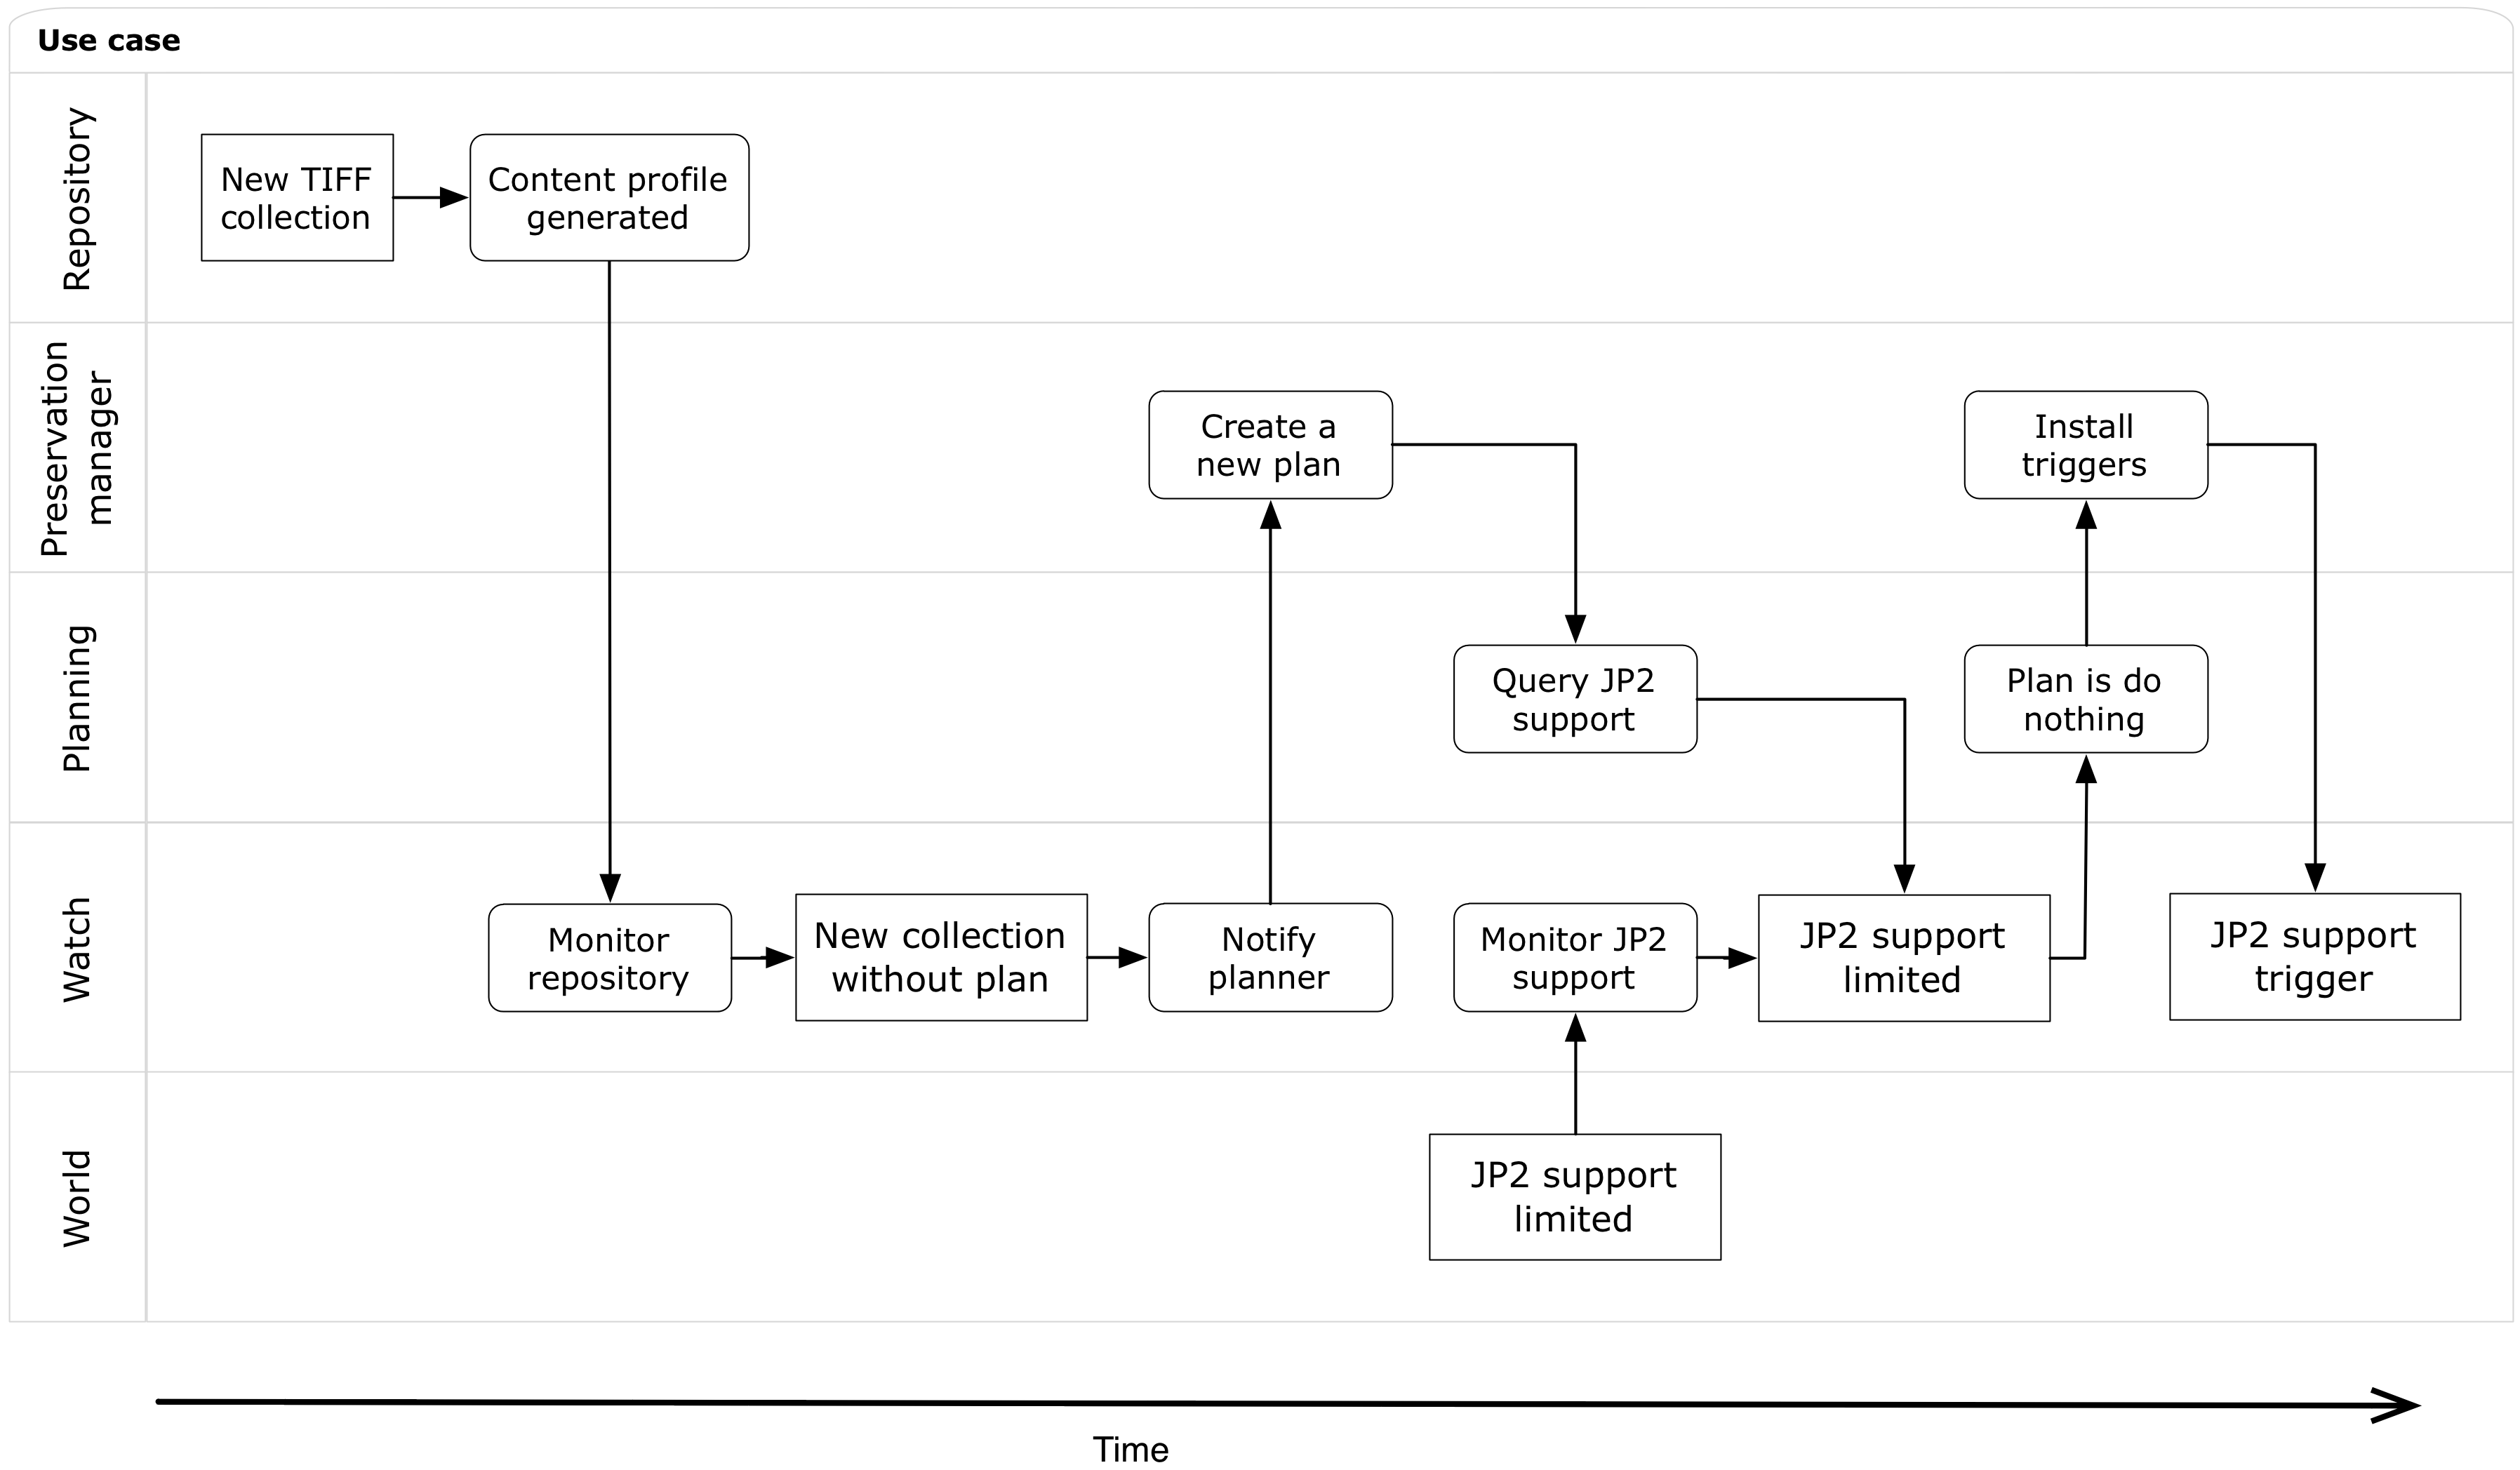
\includegraphics[width=6in]{figures/related/swimlane_step1.png}
\caption{The first step of an example preservation planning use case and the interaction between the different components through time.}
\label{fig:swimlane_step1}
\end{center}
\end{figure}

In this example an image collection that is TIFF 5.0 formatted is examined and a potential migration to the JP2 format is considered during planning. The different components that take part in this scenario are the repository, which manages the collections and provides a profile, the preservation manager, who is a human actor that has the expertise to take valid preservation decisions, a planning tool, which supports the preservation manager in his activities, a watch component, which is a monitor of internal and external activities and the world, which represents all preservation related information internal and external to the planning environment.

Figure \ref{fig:swimlane_step1} shows that the collection is ingested within the repository and a content profile is created.

Afterwards the monitoring component catches the new ingest event and collects the aggregated content profile. The monitor detects that this new collection does not have an associated plan and notifies the responsible planner.

The preservation expert creates a new plan and checks the requirements and policies of the organisation. Assume that one of the objectives is to use only formats that have widespread tool support. In this case the JP2 format still has a limited support, which results in a plan recommendation to keep the status quo. The preservation manager then installs some triggers to the monitoring component that starts observing its sources for changes in the tool support of the JP2 format.

The monitor continues its work and periodically checks for changes in the JP2 format tool support.

Assume for the sake of the example that at some future point in time (Figure \ref{fig:swimlane_step2}) the JP2 format becomes more popular and thus the number of tools that can produce and render it grows. The monitor component will catch this change and will notify the planner that there is a plan about a certain TIFF collection that needs to be re-evaluated.

\begin{figure}[th]
\begin{center}
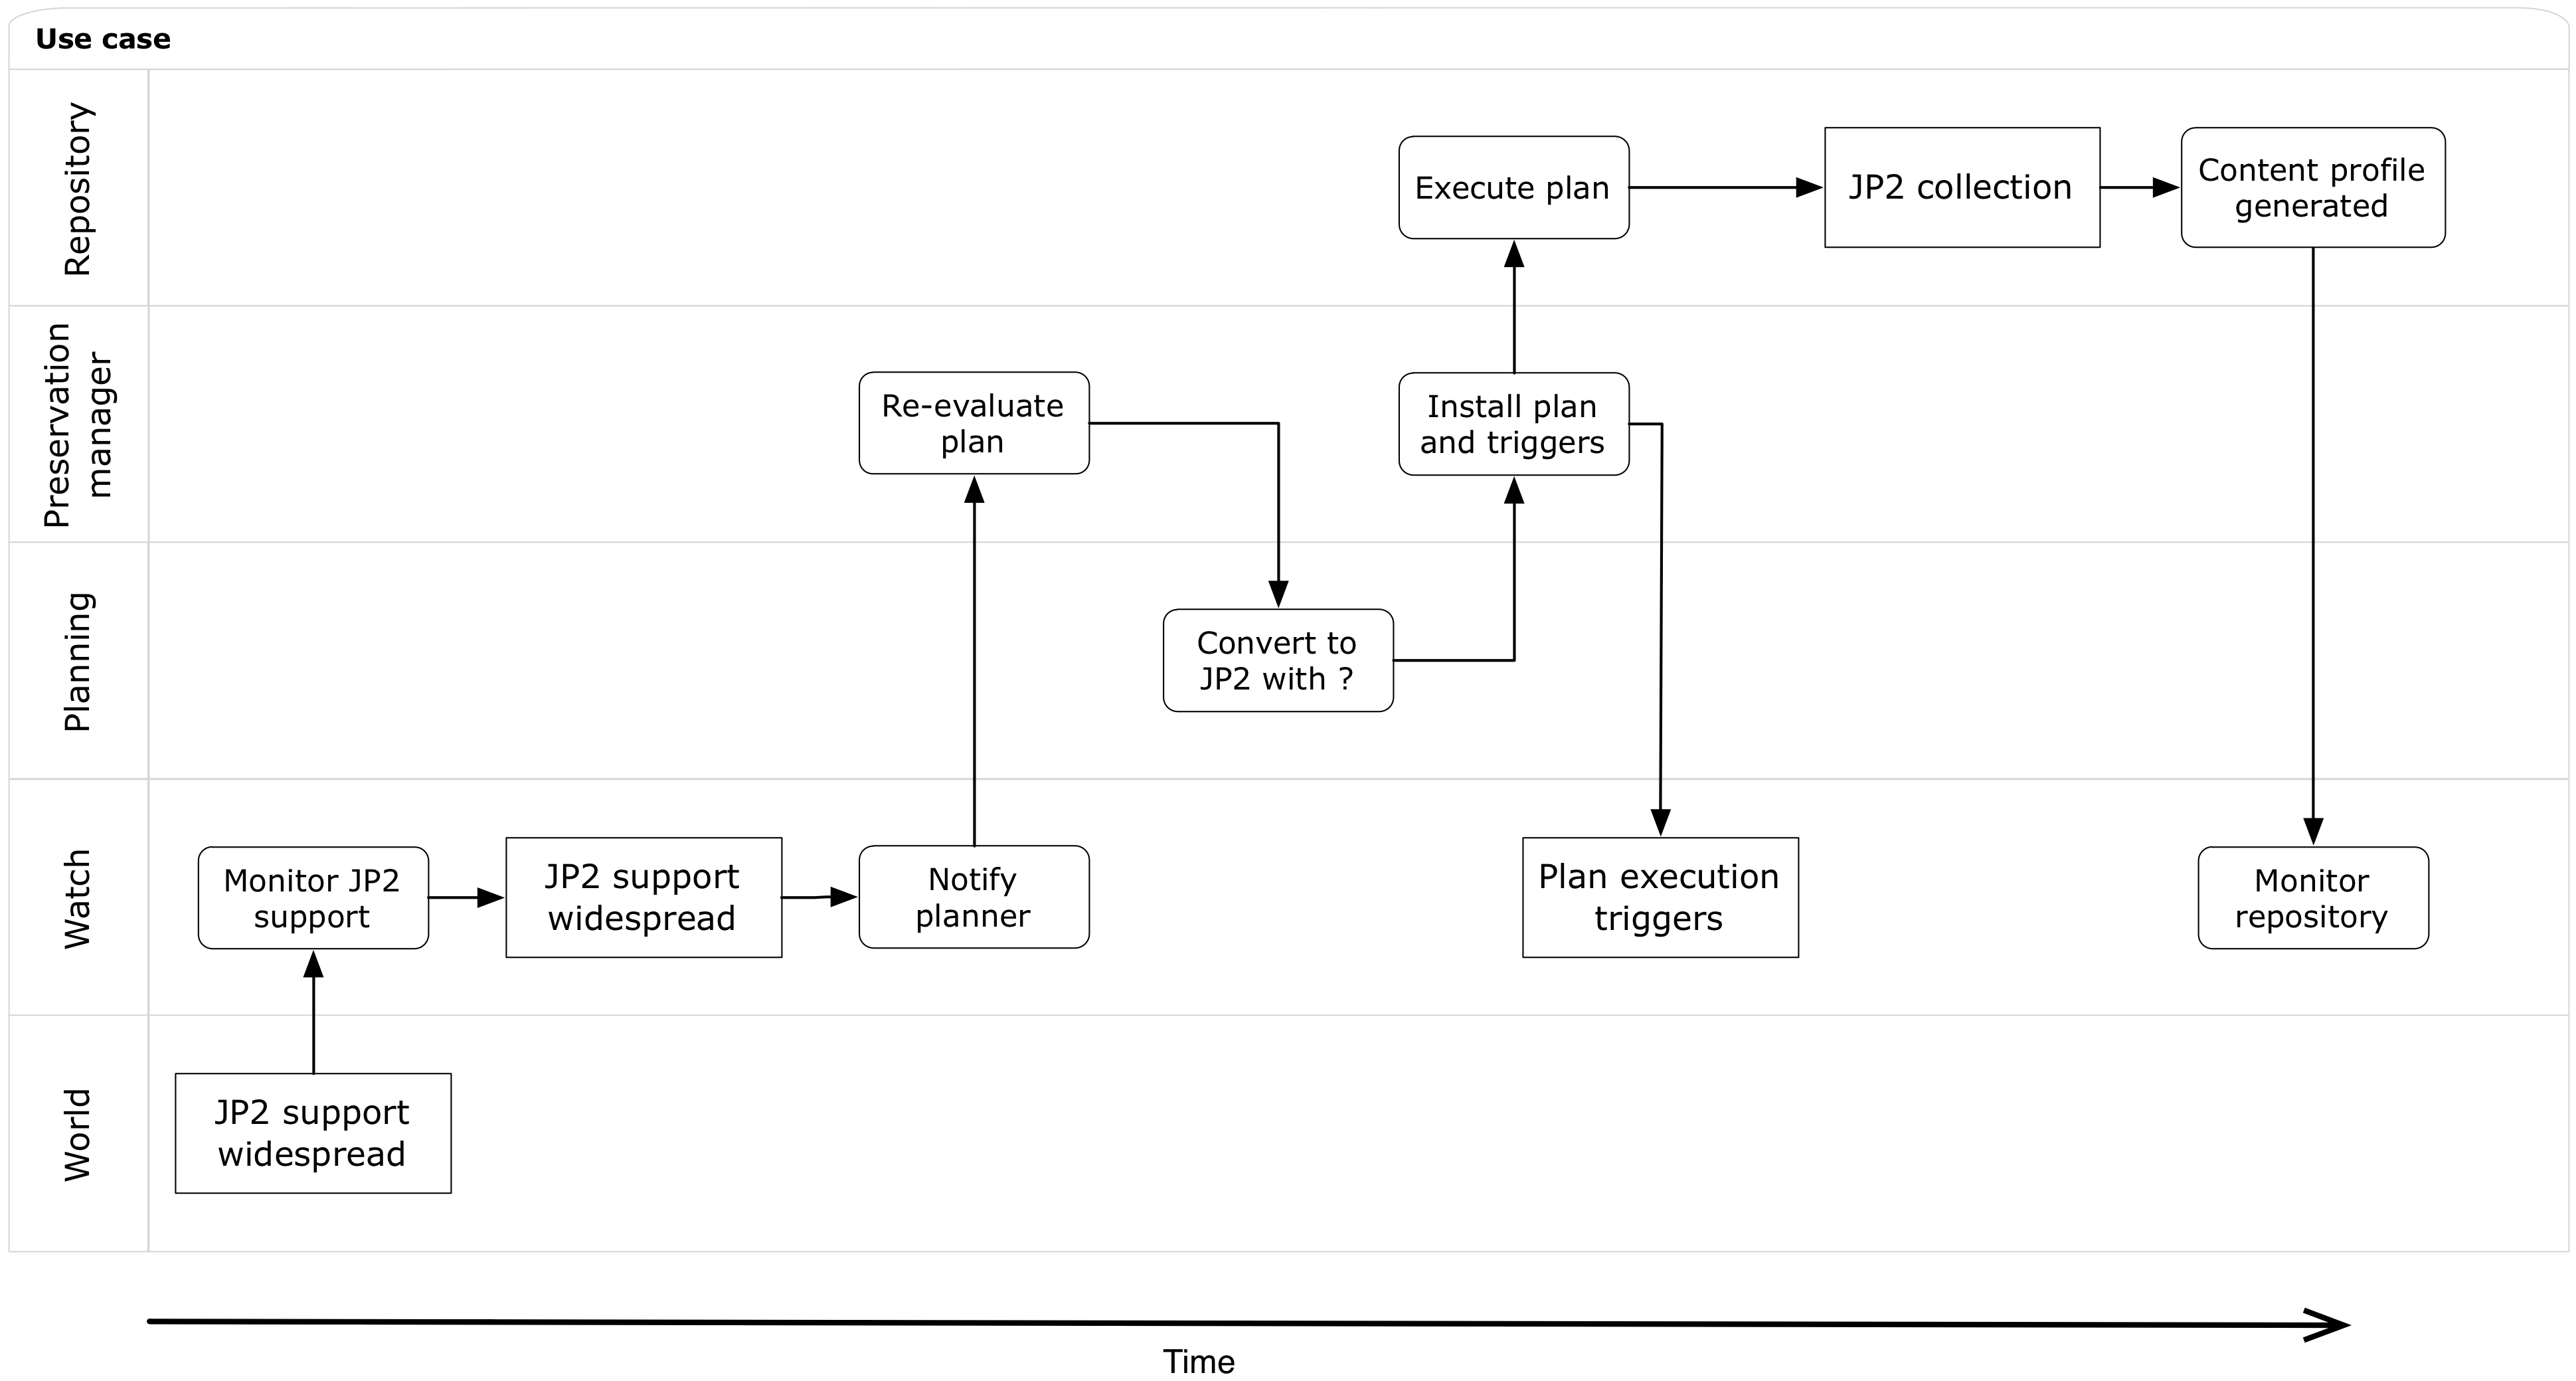
\includegraphics[width=6in]{figures/related/swimlane_step2.png}
\caption{The second step of an example preservation planning use case and the interaction between the different components through time.}
\label{fig:swimlane_step2}
\end{center}
\end{figure}

The preservation manager will conduct experiments and will create a preservation action plan that will be deployed within the repository. Before execution starts, additional triggers are installed within the monitoring component that keep track of the execution of the migration within the repository.

Once the repository executes the migration from TIFF 5.0 to JP2, the new collection is profiled again and the monitor obtains its new information and continues its work. Thus the whole lifecycle is completed.

This realistic example is summarised in the following simple list of more general steps, which usually apply to many real-world scenarios in the following order:

\begin{enumerate}
\item Organisational policies about the management of the content are created and curated.
\item A monitoring component is used to observe the policies and operations over the content within a repository for violations.
\item As part of the repository ingest, an identification and deep characterisation process extracts valuable meta data and stores it within the repository.
\item A content profile is generated and exported for other tools.
\item A monitoring component identifies that a certain subset of objects violates the policies and notifies a planning expert for the potential threat.
\item A planner uses the content profile, a profiler to analyse and stratify the content into smaller homogeneous partitions as well as identify representative sample objects for the partitions.
\item A planning tool is used to validate the threat and to create an action plan that is able to cope with the policy violations.
\item The action plan is submitted to a repository, which knows how to execute the described preservation action.
\item The monitoring component observes the operations of the repository and notifies the interested parties of important events, such as throughput, failures and task executions. 
\item The violation is taken care of and the monitor component continues its work.
\end{enumerate}

The state of the art provides some of these components and actors in this high-level workflow. Any organisation actively doing digital preservation has its own set of policies of how to handle different types of content. The problem here is that often such policies are just high-level descriptive statements, which are not structured in any specific form and thus are not machine readable. This makes it almost impossible to use in automated fashion.

Also there are numerous repositories that can manage digital objects and keep them accessible over time. They have the capabilities to extract meta data from them.

The planning tool PLATO provides the needed facilities to create an action plan and support the decision making of a preservation expert.

However, a couple of components are missing. A preservation monitor that scans relevant properties of the world and evaluates their values for changes, eventually notifying users or other agents of interesting events. Such a monitor is currently developed within the SCAPE Project \cite{becker-ipres2012, duretec:2012:watch}.

Another crucial part that is missing is a method able to profile a massive content set and stratify it into smaller homogeneous and manageable partitions. It can run within the repository or even external to it, but has to provide external interfaces for integration with planning and monitoring. Such a framework will support analysis and content stratification and thus provide better foundation for planning experiments with reduced bias.